This lab was an introduction to the usage of OpenSSL to
encrypt and decrypt data using the DES and AES256 symmetric encryption algorithms,
as well as RSA private keys used in asymmetric encryption and how to generate and gather
public and private keys, alongside message digests.

\section{Version checking and ciphers}\label{sec:version}
To check the installed version of OpenSSL, "openssl version" can be executed.
The provided virtual machine from \href{https://moodle.bcu.ac.uk/mod/url/view.php?id=7914090}{the CMP5329 Moodle page}
uses OpenSSL version 1.1.1f, dated 31st March 2020.

\begin{figure}[H]
    \centering
    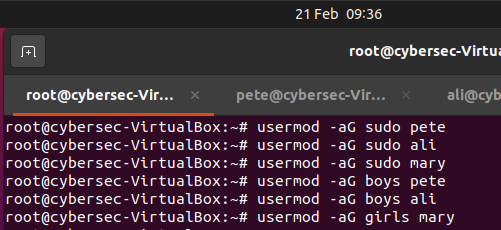
\includegraphics[width=.9\linewidth]{lab1/2}
    \caption{Getting the OpenSSL version}
    \label{fig:version}
\end{figure}

The list of OpenSSL ciphers can be viewed via "openssl ciphers".

\begin{figure}[H]
    \centering
    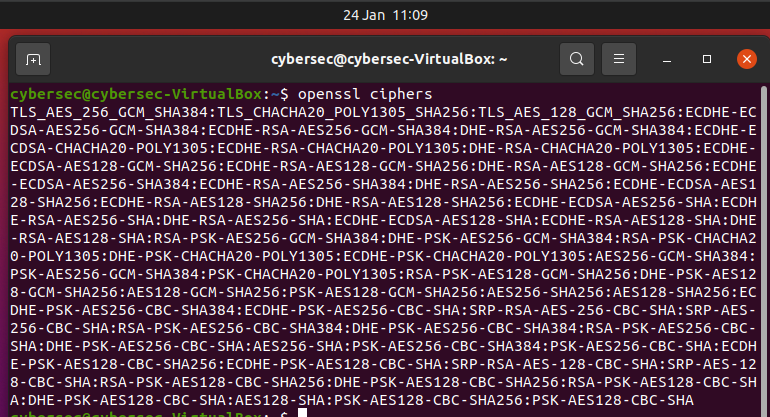
\includegraphics[width=.9\linewidth]{lab1/3}
    \caption{Getting the OpenSSL ciphers}
    \label{fig:ciphers}
\end{figure}

\section{Symmetric encryption}\label{sec:symmEncrypt}
Symmetric cryptography refers to the process of transferring data that has been encrypted by a single key.
Both the sender and receiver of this data use the same key to encrypt and decrypt the data.

\subsection{DES symmetric encryption}\label{subsec:des}
OpenSSL can be used to encrypt plaintext into ciphertext.
Many algorithms exist to generate ciphertext, but the DES symmetric encryption algorithm will be used here.

\begin{figure}[H]
    \centering
    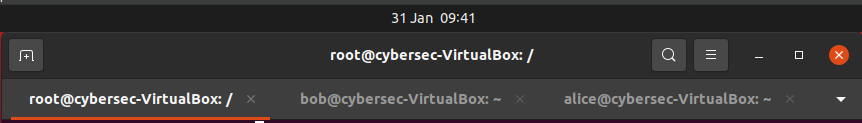
\includegraphics[width=.9\linewidth]{lab1/4}
    \caption{Converting "a secret message" to ciphertext using DES with key "secretkey".}
    \label{fig:DESEncrypt}
\end{figure}

This ciphertext can then be decoded if you know the key it was encoded with.

\begin{figure}[H]
    \centering
    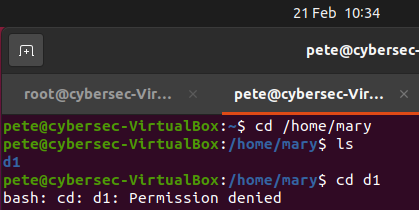
\includegraphics[width=.9\linewidth]{lab1/5}
    \caption{Decoding the ciphertext back to its original form using the key "secretkey".}
    \label{fig:DESDecrypt}
\end{figure}

\subsection{AES256 symmetric encryption and decryption}\label{subsec:aes256}
The DES algorithm is considered weak due to how simple it is to brute-force using today's processing power.
Newer algorithms were therefore developed, with one of these being AES\@.

I researched how to use this algorithm in OpenSSL, finding \href{https://www.madboa.com/geek/openssl/#how-do-i-simply-encrypt-a-file}{this help page}
\autocite{openSSLHelp} which provided details on encrypting text using the AES-256-cbc cipher.

\begin{figure}[H]
    \centering
    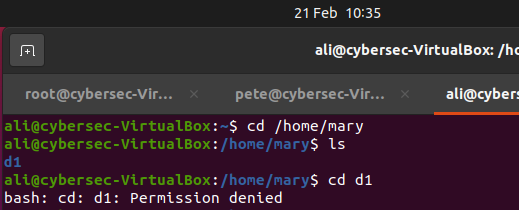
\includegraphics[width=.9\linewidth]{lab1/6}
    \caption{Encoding the plaintext with AES-256-cbc using the key "secretkey".}
    \label{fig:AESEncrypt}
\end{figure}

In this command the AES-256-cbc cipher is used, and the optional
-salt flag was added, which salts the text to provide different ciphertext.

Salting is the process of adding random data to the text prior to encoding it, which will change
the resulting ciphertext, making it harder to decrypt and increasing the strength of the encryption.

\pagebreak

\section{Asymmetric encryption}\label{sec:asymmEncryption}
Asymmetric cryptography is the practice of using two keys when transmitting data: a public key used to encrypt
data, and a private key used to decrypt it.
This is unlike symmetric encryption which uses one key for both users, but can be much more secure.
Data transferred this way has a digital signature attached, which allows for non-repudiation, as it cannot
be denied that the data originated from the user with the private key associated with the signature.
\newline

\subsection{Generating an RSA private key}\label{subsec:rsa-private-key}
OpenSSL can be used to generate these keys by using the "openssl genrsa" command.

\begin{figure}[H]
    \centering
    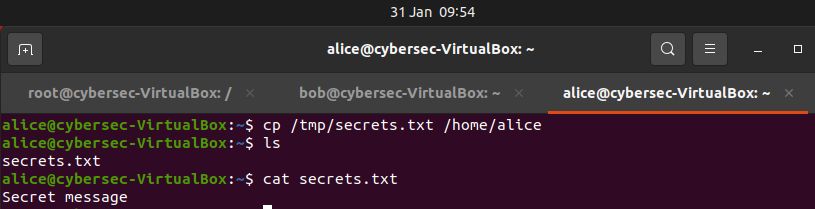
\includegraphics[width=.9\linewidth]{lab1/7}
    \caption{Generating a 2048-bit private key using genrsa.}
    \label{fig:genrsa}
\end{figure}

\pagebreak

\subsection{Storing DES3 \& passphrase encrypted RSA keys in a file}\label{subsec:storing-keys-in-file}
The key generated can then be encrypted using an encryption algorithm and a passphrase.
It can then be stored into a Privacy Enhanced Mail (.pem) file, which is
a file format 'to provide the creation and validation of digital signatures, and in addition the
encryption and decryption of signed data, based on asymmetric and symmetric cryptography.'
~\autocite[p. 1894]{PEMFormat}\\

\noindent In this example, a 1024-bit key is created using DES3 and the passphrase "secretkey".

\begin{figure}[H]
    \centering
    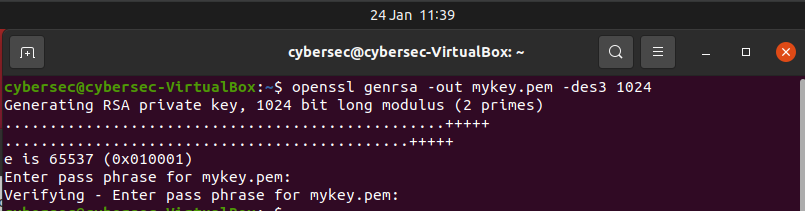
\includegraphics[width=.8\linewidth]{lab1/8}
    \caption{Generating and storing a 1024-bit private key using genrsa, DES3 and the passphrase "secretkey".}
    \label{fig:DES3Key}
\end{figure}

\begin{figure}[H]
    \centering
    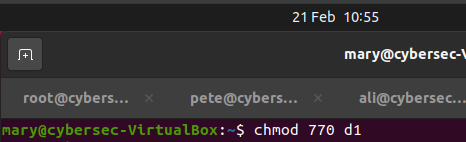
\includegraphics[width=.8\linewidth]{lab1/9}
    \caption{The key stored in mykey.pem.}
    \label{fig:mykey}
\end{figure}

\subsection{Getting a public key from the private key}\label{subsec:PubFromPriv}
The private key stored into "mykey.pem" by the previous command can be accessed again to generate a public key.

\begin{figure}[H]
    \centering
    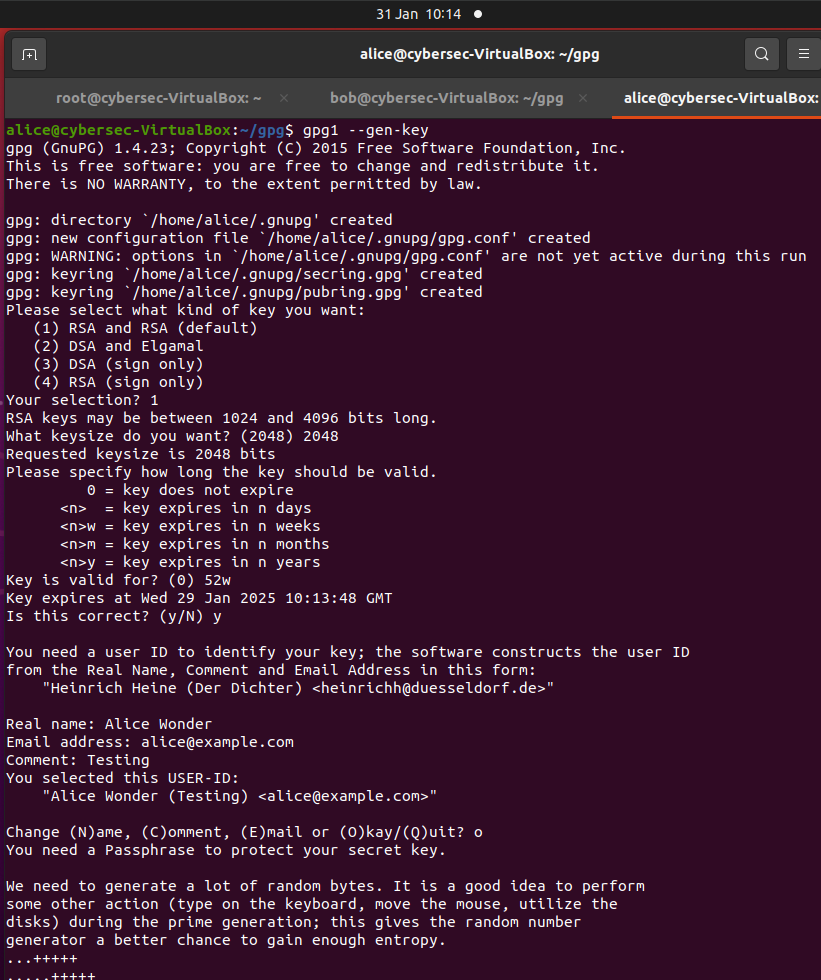
\includegraphics[width=.9\linewidth]{lab1/10}
    \caption{The public key generated from mykey.pem.}
    \label{fig:pubKey}
\end{figure}

\begin{figure}[H]
    \centering
    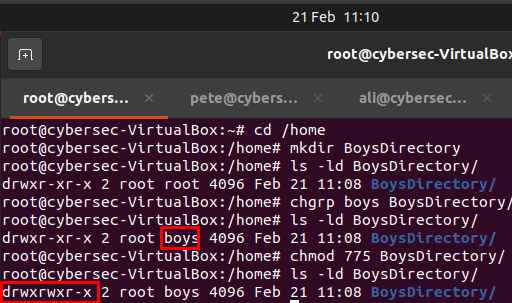
\includegraphics[width=.9\linewidth]{lab1/11}
    \caption{Storing the public key in a file.}
    \label{fig:pubKeyFile}
\end{figure}

\noindent "-out public" writes the key to a file called "public".
This file can then be read using cat.

\pagebreak

\subsection{Obtaining a message/file digest}\label{subsec:hashDigest}
To mitigate the risks of data interception or corruption, files can have "digests", which are the result
of hashing their contents.
If the file is modified whatsoever, the digest would be different.\newline

OpenSSL can generate digests using its "dgst" command.
\begin{figure}[H]
    \centering
    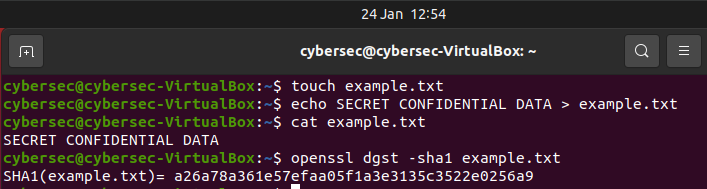
\includegraphics[width=.9\linewidth]{lab1/12}
    \caption{Creating a file, then getting the SHA1 digest of it.}
    \label{fig:digest}
\end{figure}

This can also be verified by using sha1sum, which returns the same digest.

\begin{figure}[H]
    \centering
    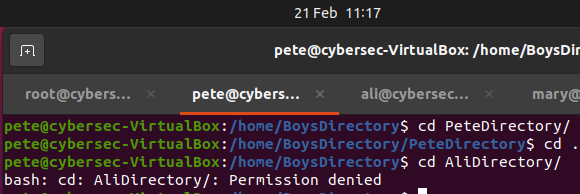
\includegraphics[width=.9\linewidth]{lab1/13}
    \caption{Verifying the digest.}
    \label{fig:digestVerify}
\end{figure}

\pagebreak

\subsection{Signing a digest}\label{subsec:SignDigest}
Signing a message digest using your private key definitively proves you sent it,
meaning that it cannot be denied that the file was sent, nor who it was sent by.

The previously used "example.txt" can again be used here to generate a digest encrypted using the "mykey.pem"
private key established earlier, which signs the digest.

\begin{figure}[H]
    \centering
    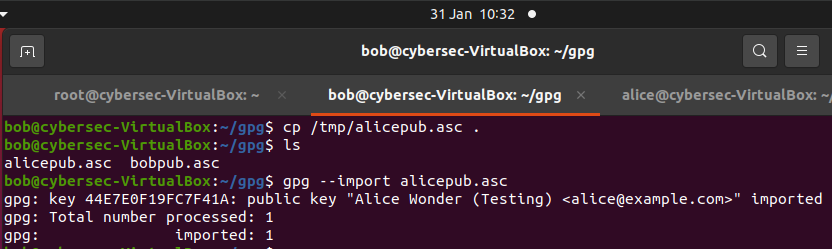
\includegraphics[width=.9\linewidth]{lab1/14}
    \caption{Writing a signed digest to a file.}
    \label{fig:writeDigest}
\end{figure}

Note that when we try to read this file, it is completely illegible, as it is not in Base64/ASCII format.
It can be converted to Base64 using OpenSSL's "enc" command.

\begin{figure}[H]
    \centering
    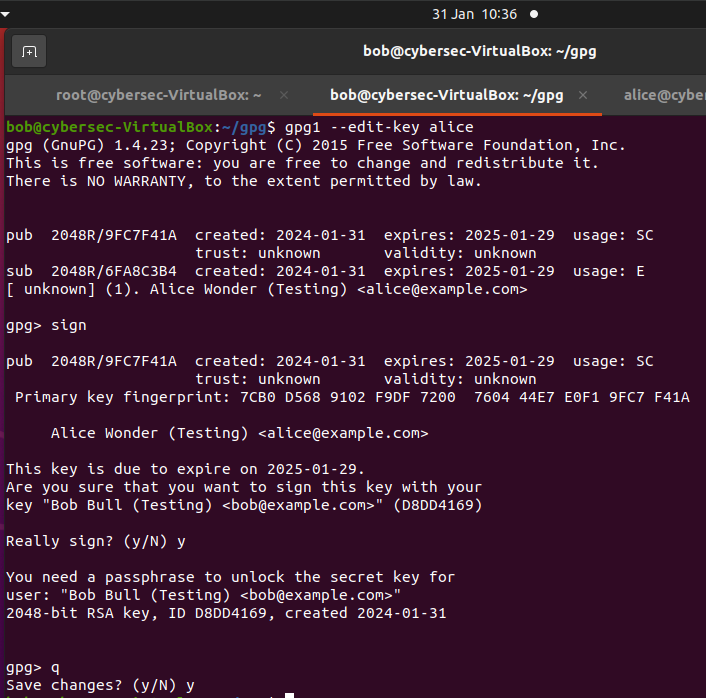
\includegraphics[width=.9\linewidth]{lab1/15}
    \caption{Encoding the signed digest to Base64.}
    \label{fig:base64Digest}
\end{figure}

Now that we have the signed digest, it can be verified using the public key, which confirms the authenticity
of the data in example.txt.

\begin{figure}[H]
    \centering
    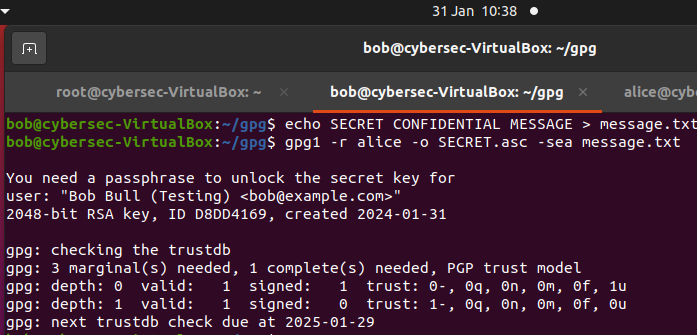
\includegraphics[width=.9\linewidth]{lab1/16}
    \caption{Verifying the signature of example.txt.}
    \label{fig:signatureVerify}
\end{figure}

This returns "Verified OK" as intended.
If the file does get modified through either corruption or a threat agent's interference,
the digest would not be the same, seen below:

\begin{figure}[H]
    \centering
    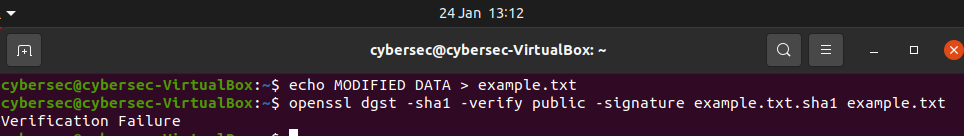
\includegraphics[width=.9\linewidth]{lab1/17}
    \caption{Failing to verify the signature of example.txt, as it has been modified.}
    \label{fig:signatureVerifyFail}
\end{figure}
